\documentclass[spec, och, labwork]{shiza}
% параметр - тип обучения - одно из значений:
%    spec     - специальность
%    bachelor - бакалавриат (по умолчанию)
%    master   - магистратура
% параметр - форма обучения - одно из значений:
%    och   - очное (по умолчанию)
%    zaoch - заочное
% параметр - тип работы - одно из значений:
%    referat    - реферат
%    coursework - курсовая работа (по умолчанию)
%    diploma    - дипломная работа
%    pract      - отчет по практике
% параметр - включение шрифта
%    times    - включение шрифта Times New Roman (если установлен)
%               по умолчанию выключен
\usepackage{subfigure}
\usepackage{tikz,pgfplots}
\pgfplotsset{compat=1.5}
\usepackage{float}

%\usepackage{titlesec}
\setcounter{secnumdepth}{4}
%\titleformat{\paragraph}
%{\normalfont\normalsize}{\theparagraph}{1em}{}
%\titlespacing*{\paragraph}
%{35.5pt}{3.25ex plus 1ex minus .2ex}{1.5ex plus .2ex}

\titleformat{\paragraph}[block]
{\hspace{1.25cm}\normalfont}
{\theparagraph}{1ex}{}
\titlespacing{\paragraph}
{0cm}{2ex plus 1ex minus .2ex}{.4ex plus.2ex}

% --------------------------------------------------------------------------%


\usepackage[T2A]{fontenc}
\usepackage[utf8]{inputenc}
\usepackage{graphicx}
\graphicspath{ {./images/} }
\usepackage{tempora}

\usepackage[sort,compress]{cite}
\usepackage{amsmath}
\usepackage{amssymb}
\usepackage{amsthm}
\usepackage{fancyvrb}
\usepackage{listings}
\usepackage{listingsutf8}
\usepackage{longtable}
\usepackage{array}
\usepackage[english,russian]{babel}

% \usepackage[colorlinks=true]{hyperref}
\usepackage{url}

\usepackage{underscore}
\usepackage{setspace}
\usepackage{indentfirst} 
\usepackage{mathtools}
\usepackage{amsfonts}
\usepackage{enumitem}
\usepackage{tikz}
\usepackage{minted}

\usepackage{booktabs}

\newcommand{\eqdef}{\stackrel {\rm def}{=}}
\newcommand{\specialcell}[2][c]{%
\begin{tabular}[#1]{@{}c@{}}#2\end{tabular}}

\renewcommand\theFancyVerbLine{\small\arabic{FancyVerbLine}}

\newtheorem{lem}{Лемма}

\begin{document}

% Кафедра (в родительном падеже)
\chair{}

% Тема работы
\title{Аналого-цифровой преобразователь}

% Курс
\course{3}

% Группа
\group{331}

% Факультет (в родительном падеже) (по умолчанию "факультета КНиИТ")
\department{факультета КНиИТ}

% Специальность/направление код - наименование
%\napravlenie{09.03.04 "--- Программная инженерия}
%\napravlenie{010500 "--- Математическое обеспечение и администрирование информационных систем}
%\napravlenie{230100 "--- Информатика и вычислительная техника}
%\napravlenie{231000 "--- Программная инженерия}
\napravlenie{10.05.01 "--- Компьютерная безопасность}

% Для студентки. Для работы студента следующая команда не нужна.
% \studenttitle{Студентки}

% Фамилия, имя, отчество в родительном падеже
\author{Стаина Романа Игоревича и Токарева Никиты Сергеевича}

% Заведующий кафедрой
% \chtitle{} % степень, звание
% \chname{}

%Научный руководитель (для реферата преподаватель проверяющий работу)
\satitle{аспирант} %должность, степень, звание
\saname{А. А. Мартышкин}

% Руководитель практики от организации (только для практики,
% для остальных типов работ не используется)
% \patitle{к.ф.-м.н.}
% \paname{С.~В.~Миронов}

% Семестр (только для практики, для остальных
% типов работ не используется)
%\term{8}

% Наименование практики (только для практики, для остальных
% типов работ не используется)
%\practtype{преддипломная}

% Продолжительность практики (количество недель) (только для практики,
% для остальных типов работ не используется)
%\duration{4}

% Даты начала и окончания практики (только для практики, для остальных
% типов работ не используется)
%\practStart{30.04.2019}
%\practFinish{27.05.2019}

% Год выполнения отчета
\date{2022}

\maketitle

% Включение нумерации рисунков, формул и таблиц по разделам
% (по умолчанию - нумерация сквозная)
% (допускается оба вида нумерации)
% \secNumbering

%-------------------------------------------------------------------------------------------

\section*{Цель работы:}

Ознакомление с принципом работы и испытание интегрального 8"=разрядного
аналого"=цифрового преобразователя.

\subsection*{Задание 1.}

Построим схему для испытания аналого-цифрового преобразователя с ЦАП.

\begin{figure}[H]
    \centering
    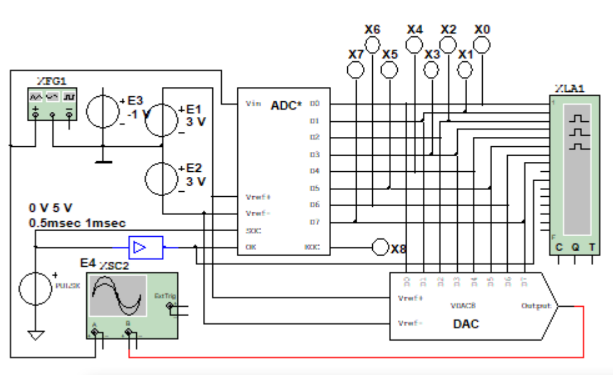
\includegraphics[width=4.96458in,height=3.03706in]{image1.png}
\end{figure}

В схему включены:

\begin{table}[H]
    \centering
    \begin{longtable}[]{@{}
    |>{\raggedright\arraybackslash}p{(\columnwidth - 4\tabcolsep) * \real{0.3333}}
    |>{\raggedright\arraybackslash}p{(\columnwidth - 4\tabcolsep) * \real{0.3333}}
    |>{\raggedright\arraybackslash}p{(\columnwidth - 4\tabcolsep) * \real{0.3333}}@{}|}
    \hline
    \begin{minipage}[b]{\linewidth}\raggedright
    Прибор
    \end{minipage} & \begin{minipage}[b]{\linewidth}\raggedright
    Тип прибора
    \end{minipage} & \begin{minipage}[b]{\linewidth}\raggedright
    Количество
    \end{minipage} \\
    \hline
    \endhead
    Генератор & Е4 & 1 \\ \hline
    Осциллограф & XSC1 & 1 \\ \hline
    Функциональный генератор & XFG1 & 1 \\ \hline
    Источник опорного напряжения & Е1, Е2 & 2 \\ \hline
    Пробники & Х0-Х7 & 8 \\ \hline
    Логический анализатор & XLA1 & 1 \\ \hline
    ЦАП & DAC & 1 \\ \hline
    8-разрядный АЦП & ADC & 1 \\ \hline
    \end{longtable}
\end{table}

\subsection*{Задание 2.}

Таблица результатов измерений:

\begin{table}[H]
    \centering
    \begin{longtable}[]{@{}
    |>{\raggedright\arraybackslash}p{(\columnwidth - 14\tabcolsep) * \real{0.0965}}
    |>{\raggedright\arraybackslash}p{(\columnwidth - 14\tabcolsep) * \real{0.1663}}
    |>{\raggedright\arraybackslash}p{(\columnwidth - 14\tabcolsep) * \real{0.1430}}
    |>{\raggedright\arraybackslash}p{(\columnwidth - 14\tabcolsep) * \real{0.1012}}
    |>{\raggedright\arraybackslash}p{(\columnwidth - 14\tabcolsep) * \real{0.1392}}
    |>{\raggedright\arraybackslash}p{(\columnwidth - 14\tabcolsep) * \real{0.0947}}
    |>{\raggedright\arraybackslash}p{(\columnwidth - 14\tabcolsep) * \real{0.1392}}
    |>{\raggedright\arraybackslash}p{(\columnwidth - 14\tabcolsep) * \real{0.1399}}@{}|}
    \hline
    \begin{minipage}[b]{\linewidth}\raggedright
    U\textsubscript{вx}, B
    \end{minipage} & \begin{minipage}[b]{\linewidth}\raggedright
    U\textsubscript{выx(цап)}, B
    \end{minipage} & \begin{minipage}[b]{\linewidth}\raggedright
    D\textsubscript{(2)}
    \end{minipage} & \begin{minipage}[b]{\linewidth}\raggedright
    D\textsubscript{(16)}
    \end{minipage} & \begin{minipage}[b]{\linewidth}\raggedright
    D\textsubscript{(10)инв}
    \end{minipage} & \begin{minipage}[b]{\linewidth}\raggedright
    D\textsubscript{(10)}
    \end{minipage} & \begin{minipage}[b]{\linewidth}\raggedright
    D\textsubscript{(10)расч}
    \end{minipage} & \begin{minipage}[b]{\linewidth}\raggedright
    $\Delta U$\%
    \end{minipage} \\
    \hline
    \endhead
    0,1 & 0,0938 & 10000101 & 85 & 133 & 5 & 5,12 & 6,25 \\ \hline
    0,2 & 0,2042 & 10001010 & 8A & 138 & 10 & 10,24 & 2,1 \\ \hline
    0,5 & 0,5158 & 10011010 & 9A & 154 & 26 & 25,6 & 3,12 \\ \hline
    1 & 0,9645 & 10110011 & B3 & 179 & 51 & 51,2 & 3,56 \\ \hline
    1,5 & 1,5042 & 11001101 & CD & 205 & 77 & 76,8 & 0,28 \\ \hline
    2 & 2,017 & 11100110 & E6 & 230 & 102 & 102,4 & 0,85 \\ \hline
    2,4 & 2,393 & 11111011 & FB & 251 & 123 & 122,88 & 0,3 \\ \hline
    -0,5 & -0,5042 & 01100110 & 66 & 102 & -26 & -25,6 & 1,5 \\ \hline
    -1 & -0,9844 & 01001101 & 4D & 77 & -51 & -51,2 & 3,56 \\ \hline
    -2 & -2,009 & 00011010 & 1A & 25 & -102 & -102,5 & 0,46 \\ \hline
    \end{longtable}
\end{table}

\subsection*{Задание 3.}

Осциллограммы и характеристики приборов:

\begin{figure}[H]
    \centering
    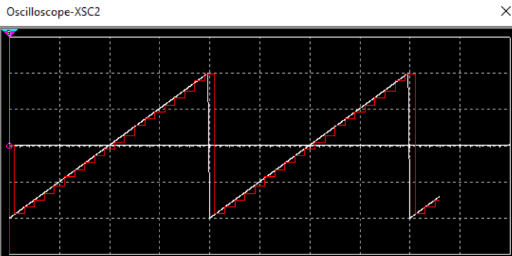
\includegraphics[width=5.33333in,height=2.66667in]{image2.png}
\end{figure}

\begin{figure}[H]
    \centering
    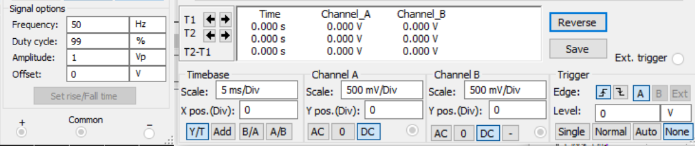
\includegraphics[width=6.49653in,height=1.30833in]{image3.png}
\end{figure}

\begin{figure}[H]
    \centering
    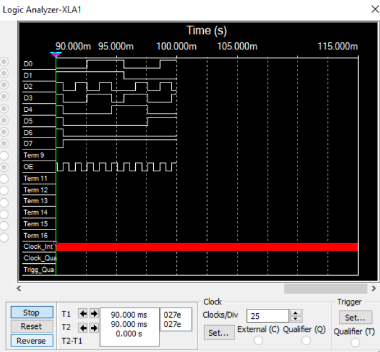
\includegraphics[width=3.95833in,height=3.66667in]{image4.png}
\end{figure}

Векторные и топографические диаграммы, графики:

\begin{figure}[H]
    \centering
    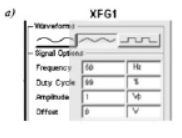
\includegraphics[width=1.89583in,height=1.4375in]{image5.png}
\end{figure}

\begin{figure}[H]
    \centering
    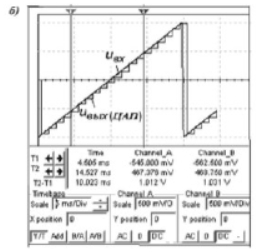
\includegraphics[width=2.69792in,height=2.625in]{image6.png}
\end{figure}

\begin{figure}[H]
    \centering
    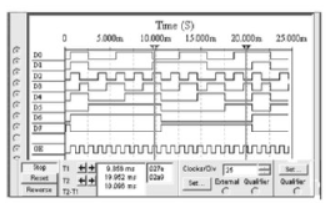
\includegraphics[width=3.42708in,height=2.21875in]{image7.png}
\end{figure}

\subsection*{Задание 4.}

\begin{figure}[H]
    \centering
    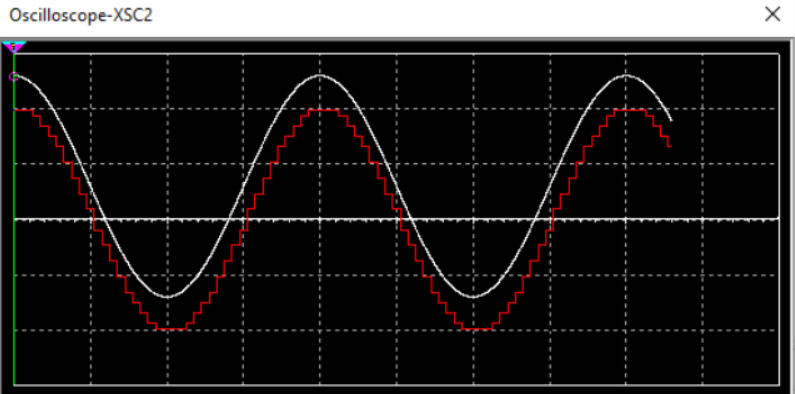
\includegraphics[width=6.49653in,height=3.21944in]{image8.png}
\end{figure}

\begin{figure}[H]
    \centering
    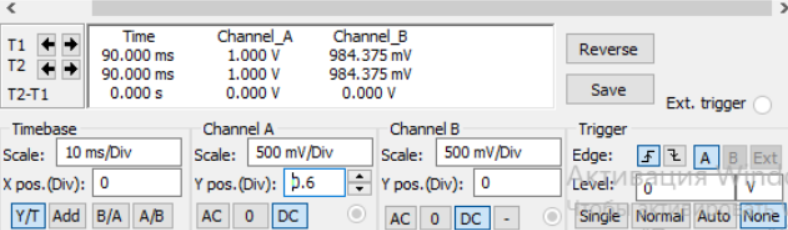
\includegraphics[width=4.63333in,height=1.89653in]{image9.png}
\end{figure}

\textbf{Вывод}: ознакомились с принципами работы АЦП и испытали
интегральный 8-разрядный аналого-цифровой преобразователь.


\section*{Тестовые задания к работе 36}

\begin{enumerate}
    \item
        Укажите \textbf{назначение} АЦП:

        Ответ: для преобразования постоянного напряжения, заданного на тактовом
        интервале, в двоичный код.
    
    \item
        Укажите \textbf{формулу Котельникова}, с помощью которой
        определяют шаг дискретизации $\Delta t$ аналогового сигнала ($f_m$ "---
        максимальная частота спектра аналогового сигнала; $t_\text{вх}$ "---
        длительность аналогового сигнала; $N$ "--- число уровней квантования):

        Ответ: $\Delta t \leq 1/2 f_m$.
    
    \item
        Определите понятие \textbf{<<абсолютная разрешающая
        способность>>} АЦП:

        Ответ: это среднее значение минимального изменения входного сигнала,
        обусловливающего увеличение или уменьшение выходного кода на единицу.

    \item
        Укажите, можно ли подавать на входы $V_\text{ref+}$ и
        $V_\text{ref–}$ АЦП \textbf{разные} (по модулю) \textbf{напряжения}:

        Ответ: да.
    
    \item
        Укажите, можно ли \textbf{свести к нулю} погрешность квантования
        аналогового сигнала посредством выбора параметров устройства, например
        за счет увеличения разрядности АЦП:
    
        Ответ: нет.

    \item
        Укажите,какую \textbf{погрешность} квантования имеет
        8"=разрядный АЦП при напряжениях на входах $V_\text{ref+} = 2$ В,
        $V_\text{ref–} = 0$ и отсчете входного напряжения $u_\text{вх}(k \Delta
        t) = 1$ В:

        Ответ: $\pm 3.9$ мВ

    \item
        Укажите \textbf{десятичный эквивалент} двоичного кода на выходе
        8"=разрядного АЦП, если опорные напряжения $V_\text{ref+} = 2$ В,
        $V_\text{ref-} = -2$ В, а входное напряжение $u_\text{вх} = 0.5$ В:

        Ответ: 32.

    \item
        Выберите из приведенных ниже значений минимально необходимые
        \textbf{значения опорных напряжений} $\pm V_\text{ref}$ для
        преобразования синусоидального напряжения $u_\text{вх}(t) = 1.41 \sin
        \omega t$:
    
        Ответ: $\pm 2$ В.

    \item
        Укажите значение расчетного \textbf{шестнадцатеричного кода}
        16"=разрядного АЦП,если на его вход подано напряжение $u_\text{вх}(k
        \Delta t) = 0.25$ В при $\pm V_\text{ref} = \pm 2$ В:
    
        Ответ: 1000.

    \item
        Укажите \textbf{выражение}, с помощью которого определяют
        десятичный эквивалент двоичного кода на выходе 14"=разрядного АЦП:

        Ответ: $D = 4096 u_\text{вх} / (V_\text{ref+} + |-V_\text{ref-}|)$.
    
    \item
        Укажите, как изменится \textbf{выходной код} АЦП при неизменном
        входном $u_\text{вх}$ и опорных напряжениях $V_\text{ref+} = 2$ В и
        $V_\text{ref-} = -2$ В, если установить $V_\text{ref-} = 0$:
    
        Ответ: его значение уменьшится в 2 раза.

    \item
        Укажите характер изменения \textbf{общей погрешности}
        преобразования входного сигнала при увеличении разрядности АЦП:
    
        Ответ: погрешность преобразования уменьшится.
 
    \item
        Укажите перспективные \textbf{направления} развития АЦП:
    
        Ответ:

        \begin{itemize}
            \item повышение быстродействия основных узлов АЦП, в частности компараторов;
            \item применение стабилизированных источников опорного напряжения;
            \item использование микропроцессоров в преобразователях.
        \end{itemize}

    \item
        Укажите, какие \textbf{операции} необходимо выполнить при
        аналого"=цифровом преобразовании:
    
        Ответ: дискретизацию по времени аналогового сигнала, квантования по уровню его
        отсчетов и кодирование квантованных уровней.

    \item
        Укажите, обладает ли способ последовательного счета
        аналого"=цифрового преобразования наибольшим быстродействием:
    
        Ответ: да.
\end{enumerate}

\end{document}
